\documentclass[a4paper]{article}

\setlength{\parskip}{0.1em}
\usepackage{caratula}
\usepackage[utf8]{inputenc}
\usepackage[T1]{fontenc}
\usepackage[spanish,es-tabla]{babel}
\usepackage{amsmath}
\usepackage{mathtools}
\usepackage{csquotes}
\usepackage{IEEEtrantools}
\usepackage{amssymb}
\usepackage{amsfonts}
\usepackage{fancyhdr}
\usepackage{pdfpages}
\usepackage{listings}
\usepackage{xcolor}
\usepackage{float}
\usepackage{inputenc}
\usepackage{subcaption}

\lstset { %
    language=C++,
    backgroundcolor=\color{white}, % set backgroundcolor
    basicstyle=\footnotesize,% basic font setting
}

\pagestyle{fancyplain}
% Encabezado
\lhead{Métodos Numéricos}

\begin{document}
\titulo{Trabajo Práctico III}
\subtitulo{Reconstrucción de Imágenes}
\fecha{2 de Diciembre de 2018}
\materia{Métodos Numericos}

\integrante{Carreira Munich, Tobías Agustín}{278/17}{tcarreira@dc.uba.ar}
\integrante{Martino, Maximiliano}{123/17}{maxii.martino@gmail.com}
\integrante{Nahmod, Santiago Javier}{016/17}{snahmod@dc.uba.ar}
\integrante{Torres, Edén}{017/17}{eden.etorres@gmail.com}
\maketitle

% TODO: pensar estas cosas

\begin{abstract}
	Cuadrados M\'inimos Lineales (CML) es un m\'etodo com\'unmente usado para estimar valores desconocidos a partir de valores conocidos. En este trabajo evaluaremos un modelo para reconstruir im\'agenes tomogr\'aficas sujetas a ruido utilizando el mencionado m\'etodo.
\end{abstract}

\textit{Palabras clave:} Cuadrados M\'inimos Lineales (CML), Im\'agenes Tomogr\'aficas Computadas, Aproximaci\'on, Reconstrucción de Imágenes



\tableofcontents
\section{Introducción}
\label{sec:introduccion}
% Escribir contexto del problema, qué es una tomografía computada y por qué nos interesa
Cada vez se utilizan herramientas computacionales en más ramas de las ciencias, incluyendo a las ciencias médicas.
Las aplicaciones de sistemas asistidos por computadoras en distintas especialidades de estas ciencias
presentan una gran mejoría en el sistema de salud a nivel mundial\footnote{https://es.wikipedia.org/wiki/Inform\%C3\%A1tica\_en\_salud}.
El veloz avance de la computación (tanto en software como en hardware)
posibilita un constante progreso en el desarrollo de nuevas aplicaciones médicas.
Algunos de los primeros usos fueron el procesamiento de historias clínicas y datos epidemiológicos.
Luego se han agregado los instrumentos de diagnóstico y tratamiento médicos, entre otros\footnote{http://www.cocmed.sld.cu/no63/n63edi.htm}.

En el presente trabajo, nos interesa estudiar la aplicación de diferentes técnicas algorítmicas
y de aproximación para la reconstrucción de imágenes.
En particular, desarrollaremos un programa que nos permita realizar reconstrucciones de imágenes tomográficas computadas.
Estas consisten en atravesar el objeto de estudio con rayos X,
para así lograr estimar la densidad del mismo.
Las imágenes tomográficas computadas permiten analizar las estructuras internas de las distintas partes del organismo,
lo cual facilita el diagnóstico de distintos problemas médicos, como fracturas, hemorragias internas, tumores o infecciones en los distintos órganos.
También permite conocer la morfología de la médula espinal y de los discos intervertebrales
o medir la densidad ósea, importante en el caso de osteoporosis\footnote{https://www.nibib.nih.gov/science-education/science-topics/computed-tomography-ct}.

Un problema que se presenta, es que los instrumentos utilizados poseen errores de medición.
Y esto debe ser tenido en cuenta, pues por los usos descritos anteriormente un error de este tipo
podría derivar en un mal diagnóstico,
lo cual conllevaría consecuencias aún peores.
Esto nos motiva a estudiar diferentes métodos de aproximación para solventar los problemas de precisión.
En particular, analizaremos el método de cuadrados mínimos lineales.
Veremos la calidad de las reconstrucciones que consigue y la velocidad a la cual lo hace,
además de experimentar con distintos tipos de tomografías y niveles de ruido, entre otras cosas.
\section{Marco Teórico}
\label{sec:Marco Teorico}

\subsection{Contexto}
% Cosas sobre el método de reconstrucción
En el presente trabajo nos proponemos modelar un problema práctico para resolverlo utilizando métodos computacionales.
Este problema consiste en reconstruir imágenes, en particular nos interesa
poder reconstruir imágenes tomográficas sujetas a ruido.

Como se dijo en la sección \ref{sec:introduccion}, la tomografía computada, o \verb|TC|, es un procedimiento
computarizado de imágenes por rayos X con el cual, en lugar de obtener una imagen de proyección
(como hace la radiografía convencional),
se obtienen múltiples imágenes al efectuar movimientos de rotación alrededor del cuerpo
con la fuente de rayos X y los detectores de radiación.
La representación final de la imagen tomográfica se obtiene mediante
la captura de las señales por los detectores y su posterior proceso mediante algoritmos de reconstrucción,
los cuales nos proponemos profundizar.

El aparato de \verb|TC| emite un haz de rayos X que incide sobre el objeto que se estudia.
La radiación que no ha sido absorbida por el objeto es recogida por los detectores.
Luego el emisor del haz, que tenía una orientación determinada (por ejemplo, estrictamente vertical a 90º)
cambia su orientación (por ejemplo, haz oblicuo a 95º),
se realizan así múltiples disparos con diferentes ángulos para tratar de capturar todas las partes del objeto.
Luego este espectro también es recogido por los detectores\footnote{https://en.wikipedia.org/wiki/CT\_scan}.
Como además los instrumentos tienen errores de medición es preferible realizar
repetidas veces el mismo envío para tratar de disminuir estos errores de precisión asociados. 

\subsection{Modelado del problema}
Deseamos modelar el problema descrito mediante un sistema de ecuaciones lineales.
Diremos que un rayo (que está dado por una recta en el espacio)
atraviesa cierta distancia en un cierto tiempo.
Dicho tiempo dependerá de la velocidad a la cual pueda hacerlo.
A mayor densidad del objeto atravesado, menor velocidad.

Las leyes físicas nos indican que, dado una velocidad \textit{v}, tiempo \textit{t} y distancia \textit{d},

\begin{equation*}
    t = d v^{-1}
\end{equation*}

Sin embargo, esta velocidad va a variar dependiendo el objeto que este atravesando en cada instante.
Como las computadoras trabajan con sistemas discretos,
para lograr determinar dicho sistema, elegiremos
una determinada granularidad para poder representar a la imagen.
Es decir, limitaremos nuestra reconstrucción a una imagen de cierta
cantidad de píxeles, donde cada pixel representa cierto espacio.

Dada una imagen cuadrada, la cual tomaremos como fuente de verdad absoluta,
en escala de grises (es decir, con valores de 0 a 255 donde 0 representa al vacío y 255 a un objeto muy difícil de atravesar),
simulamos el proceso tomográfico ``emitiendo'' un conjunto de rayos
y midiendo su tiempo y distancia recorrida.
Se discretiza al objeto en $n x n$ celdas cuadradas.
Si llamamos $d^{k}_{ij}$ a la distancia que recorre el $k-esimo$ rayo en la celda $ij$
(es decir, la cantidad de pixeles de la imagen original por los que pasa)
y llamamos $v_{ij}$ a la velocidad de la señal del rayo en esa celda
(cumpliendo que $v^{-1}_{ij}$ es el valor del pixel en dicho lugar),
entonces el tiempo $t_{k}$ de recorrido de la señal completa es:

\begin{equation*}
    t_{k} = \sum_{i=1}^{n} \sum_{j=1}^{n} d^{k}_{ij} v^{-1}_{ij}
\end{equation*}

De esta manera, obtendremos un vector $t \in \mathbb{R}^{m}$, donde $m$ es la cantidad rayos, 
tal que la coordenada $k$ del vector $t$ indica el tiempo de recorrida de la $k-esima$ señal.

Si definimos una matriz $D \in \mathbb{R}^{mxn^{2}}$
(dado que son $m$ rayos y $n^2$ pixeles de la discretización)
con los valores $d^{k}_{ij}$ en cada fila $k$.
A partir de $D$ y $t$,
seremos capaces de reconstruir las velocidades de recorrida originales $v_{ij}$ resolviendo el sistema de ecuaciones: 

\begin{equation*}
    Ds = t    
\end{equation*}

Donde $s \in \mathbb{R}^{n^{2}}$ corresponderá a las inversas de las velocidades.
Nos interesa \textit{s} por sobre \textit{v} ya que representa la densidad del objeto en cada punto,
lo mismo que representaban los pixeles de la imagen original.

La existencia de errores de medición en el vector $t$ hará que nuestro sistema resulte incompatible, 
es decir que no será posible hallar un vector solución $s$. Para tratar este problema,
resolveremos el sistema $Ds = t$ mediante el método de aproximación por cuadrados mínimos lineales, descripto más adelante en la sección \ref{sec:cml}, obteniendo así una solución que resuelve de forma aproximada el sistema original.


\subsection{Simulación del tomógrafo}
% Por qué simulamos? Cómo se modela eso? Contar las cosas que cuenta el enunciado SIN COPY PASTE
% Ver si es mejor escribir estoy antes o despues de lo de modelado del problema

Para poder evaluar nuestro modelo de reconstrucción necesitaríamos un tomógrafo
o al menos poder contar con los datos crudos del mismo.
Ambos requisitos resultan imposibles de satisfacer,
pues contar con un tomógrafo real implicaría una gran inversión de dinero
y acceder a datos médicos e historias clínicas ajenas esta regulado por ley\footnote{http://servicios.infoleg.gob.ar/infolegInternet/anexos/160000-164999/160432/norma.htm},
sin siquiera comenzar a hablar de la continua exposición a radiación que esto conllevaría.

Por estos motivos es que tomamos la decisión de realizar una simulación de nuestro tomógrafo.
Ésta consistirá en generar datos de prueba partiendo de imágenes sintéticas que consideramos reales,
es decir, serán la sección de nuestro objeto a escanear.
Luego teniendo en cuenta el procedimiento a realizar, descrito anteriormente,
interpretaremos el valor de cada pixel de la imagen como el dato real de densidad del cuerpo,
es decir, como la velocidad (inversa) de recorrido de las señales de rayos X al atravesar ese pixel.

Siguiendo el procedimiento que describimos anteriormente, nuestro modelo de simulación
también debería ser capaz de poder simular rayos sobre la imagen real o cuerpo a escanear
de distinta forma (distintos ángulos, etc.).
Una vez definida la forma de generar rayos, debemos definir la discretización del espacio a escanear.

De esta forma, estaríamos en condiciones de poder representar diferentes clases de tomógrafos
con solo alternar la forma/dirección en que los rayos son generados y la discretización elegida,
debido a que algunos los producen de forma axial, otros paralelos, etc.

De acuerdo a lo mencionado anteriormente, primero nos encargaremos de generar los rayos
sobre la imagen real para poder medir el tiempo $t_{k}$ de cada rayo $k$
y la longitud del mismo rayo en cada celda de la grilla discretizada $d^{k}_{ij}$.

\subsection{Resolución de CML}
\label{sec:cml}
% Contar por que usamos SVD y en que consiste

\subsubsection{Utilización de CML y SVD} %porque usamos SVd?
\label{sec:intro-cml}
Como se discutió anteriormente, nuestro sistema de ecuaciones lineales estará sobredeterminado.
Lo cual en principio no debería traer problemas mayores, pero sabemos que los instrumentos
utilizados poseen error con lo cual este sistema no será un sistema compatible,
es decir, que no seremos capaces de hallar un vector $s$ que sea solución de $Ds = t$.
Por lo tanto, tendríamos que buscar una solución que aproxime de la mejor manera posible a la solución ideal del sistema.
Para ello tendremos que estudiar métodos de aproximación,
y en el presente trabajo nos proponemos evaluar el método de aproximación
por cuadrados mínimos lineales (CML)\footnote{https://en.wikipedia.org/wiki/Least\_squares}.

Con este método, en vez de resolver $Ds = t$, buscaremos minimizar

\begin{equation*}
    ||Ds - t||_{2}
    \label{eq:1}
\end{equation*}

La utilización de este método implica la resolución de las ecuaciones normales,
lo cual nos presenta un considerable problema de estabilidad numérica,
pues por lo que veremos más adelante la matriz asociada al sistema de ecuaciones normales
aumenta de manera cuadrática el número de condición que teníamos originalmente.
Para tratar de solventar este problema utilizaremos la descomposición SVD\cite{burdenSVD} de la matriz $D$,
pues podemos aplicarla para la solución de cuadrados mínimos lineales de la siguiente manera:

% Sea una matriz A $\in \mathbb{R}^{mxn}$, con $m > n$, y un vector $b \in \mathbb{R}^{m}$. El objetivo de CML es hallar un $x \in \mathbb{R}^{n}$ tal que minimice $||Ax - b||_{2}.$
Siendo $D = U \Sigma V^{t}$ la factorización SVD de $D$, y dado que $U$ y $V$ son ortogonales y preservan  norma:
\begin{equation*}
     ||Ds - t||_{2} = ||U\Sigma V^{t} s - t||_{2} = ||U^{t} (U\Sigma V^{t} s - t)||_{2} = ||\Sigma V^{t}s - U^{t}t||_{2}
\end{equation*}
Definimos $z = V^{t}s$ y $c = U^{t}t$. Luego:
\begin{equation*}
    ||Ds - t||_{2} = ||(\sigma_{1}z_{1} - c_{1},\sigma_{2}z_{2} - c_{2}, ... ,s_{k} z_{k} - c_{k} , -c_{k+1}, ... , -c_{m})^{t}||_{2}
\end{equation*}
\begin{equation*}
    = \lbrace \sum^{k}_{i=1} (\sigma_{i}z_{i} - c_{i})^{2} + \sum^{m}_{i=k+1} (c_{i})^{2} \rbrace^{1/2}
\end{equation*}
La norma se minimiza cuando el vector $z$ se elige de la siguiente forma:
\begin{equation*}
    z_{i} =
    \begin{cases}
      c_{i}/\sigma_{i} & \text{si } i \leq k \\
      arbitrario &  \text{si } k < i \leq n \\
    \end{cases}
\end{equation*}

Finalmente, debido a que $c = U^{t}b$ y $x = Vz$ son ambas f\'aciles de computar, la solución de CML es f\'acilmente hallable.
\subsection{Condicionamiento del sistema}
% Contar sobre el k2, y que debe suceder para que DtD sea SDP
Para estudiar el condicionamiento de la matriz $(D^{t}D) \in  \mathbb{R}^{mxm}$
proponemos mirar su descomposición en valores singulares (SVD):

Sea $D = U \Sigma V^{t}$ la SVD de $D$, luego:
\begin{equation*}
    D^{t}D = (U\Sigma V^{t})^{t}(U\Sigma V^{t}) = V\Sigma^{t}U^{t}U\Sigma V^{t} = V\Sigma^{t}\Sigma V^{t} 
\end{equation*}

Luego,
\begin{equation}
    D^{t}D = V\Sigma^{t}\Sigma V^{t}
\end{equation}

Ahora podemos hacer uso de la siguiente propiedad:

Dada una matriz $A \in  \mathbb{R}^{nxn}$ y sea $r = rg(A)$, su número de condición es equivalente a la siguiente expresión:
\begin{equation}
    k_{2}(A) = || A ||_{2} . || A^{-1} ||_{2} = \sigma_{1}/\sigma_{r}
\end{equation}

Por lo tanto, si queremos saber el número de condición de la matriz $D^{t}D$
debemos hallar los autovalores de la matriz $(D^{t}D)^{t}(D^{t}D)$,
pues por definición los valores singulares de la matriz $D^{t}D$
son la raíz cuadrada de los autovalores de $(D^{t}D)^{t}(D^{t}D)$.
Pero como la matriz $D^{t}D$ es una matriz semidefinida positiva y  simétrica, pues $(D^{t}D)^{t} = (D^{t}D)$,
sabemos que sus autovalores coinciden con sus valores singulares.

Luego, hallemos los autovalores de $D^{t}D$ usando el resultado obtenido en (1):

Sea $i = 1, ... , m$, veamos que pasa con $v_{i}$:
\begin{equation*}
    (D^{t}D).v_{i} = V \Sigma^{t}\Sigma V^{t}.v_{i} = V\Sigma^{t}\Sigma .e_{i} = 
    V\Sigma .\sigma_{i}.e_{i} = V.(\sigma_{i})^{2}.e_{i} = (\sigma_{i})^{2}.v_{i}
\end{equation*}

Luego, $v_{i}$ es autovector de autovalor $\lambda_{i} = (\sigma_{i})^{2}$.
Por lo tanto, obtenemos que los valores singulares de $D^{t}D$ son $\sigma\prime_{i} = \lambda_{i} = (\sigma_{i})^{2} $

Finalmente, si $r = rg(D^{t}D)$ y utilizando la propiedad (2), el número de condición de la matriz $D^{t}D$ resulta:
\begin{equation*}
     k_{2}(D^{t}D) =  \sigma\prime_{1}/\sigma\prime_{r} = (\sigma_{1})^{2}/(\sigma_{r})^{2} = (\frac{\sigma_{1}}{\sigma_{r}})^{2} 
\end{equation*}

Esto implica que al estar utilizando cuadrados m\'inimos lineales el condicionamiento de la matriz asociada al sistema de ecuaciones normales que queremos resolver empeora de manera cuadr\'atica con respecto a la matriz asociada al sistema original, pues $k_{2}(D^{t}D) = (\frac{\sigma_{1}}{\sigma_{r}})^{2} = k_{2}(D)^{2}$

Consecuentemente, si queremos que el número de condición de la matriz $D^{t}D$ resulte bajo, mirando el resultado obtenido en (2), requerimos que sus valores singulares estén todos muy próximos (el mínimo se realiza cuando $\sigma_{1} = \sigma_{r}$). 


En nuestro caso particular, como la matriz  $D^{t}D$ es simétrica semidefinida positiva, hablar de sus valores singulares es equivalente a hablar de sus autovalores. Por lo tanto, requerimos que sus autovalores sean muy parecidos, es decir que si los graficamos como puntos en la recta real estos deberían verse como una recta. Y como estamos hablando de autovalores, esto es equivalente a decir que dada una base de autovectores, al aplicarle nuestra matriz a cualquier vector de este conjunto el mismo debería achicarse o estirarse una magnitud muy similar a cualquier otro. Lo cual resulta muy improbable de que pase.\footnote{http://web.math.princeton.edu/mathlab/projects/ranmatrices/yl/randmtx.PDF}\footnote{https://en.wikipedia.org/wiki/Circular\_law} Como consecuencia, con una alta probabilidad deberemos lidiar con una matriz mal condicionada.

\subsection{Condiciones para que $D^{t}D$ sea SDP}
Por otro lado, también nos interesa ver que la matriz $D^{t}D$ es una matriz simétrica semidefinida positiva
y dar condiciones para que resulte una matriz simétrica definida positiva,
para que esto nos garantice estabilidad numérica.

Ya vimos anteriormente que $D^{t}D$ resulta una matriz simétrica, ahora veamos que resulta semidefinida positiva.

Por definición tenemos que ver que $\forall x \neq 0 \ \in \mathbb{R}^{m} \ \ x^{t}(D^{t}D)x \geq 0$\\
Veamos:
\begin{equation*}
    \forall x \neq 0 \ \in \mathbb{R}^{m} \ \ x^{t}(D^{t}D)x = (x^{t}D^{t})(Dx) = (Dx)^{t}(Dx) = ||Dx|| \geq 0
\end{equation*}

Luego nuestra matriz resulta semidefinida positiva. 

Ahora demos condiciones para que resulte definida positiva,
es decir que $\forall x \neq 0 \ \in \mathbb{R}^{m} \ \ x^{t}(D^{t}D)x > 0$

Veamos:
\begin{equation*}
    \forall x \neq 0 \ \in \mathbb{R}^{m} \ \ ||Dx|| > 0 \Leftrightarrow \nexists \ x \neq 0 \ tal  \ que \ \ Dx = 0 \Leftrightarrow Nu(D) = \lbrace0\rbrace  \Leftrightarrow rg(D) = n^{2}
\end{equation*}

Por lo tanto, para que nuestra matriz sea simétrica definida positiva es suficiente pedir que la matriz $D$ sea de rango máximo. Que es lo mismo que decir que las columnas de $D$ sean linealmente independiente, y por como esta compuesta nuestra matriz, esto resulta equivalente a pedir que haya al menos $n^{2}$ filas, conformadas por los valores $d^{k}_{ij}$, que resulten linealmente independientes.

\subsection{Aproximación de menor rango}
\label{sec:lowrank}
Una propiedad de gran importancia al usar la factorización SVD
es la de poder aproximar la matriz reduciendo la cantidad de cálculos.

Dado $D = U \Sigma V^{t}$ la factorización SVD de $D \in \mathbb{R}^{mxn}$,
dado un $r$ natural, si se particiona $U$, $\Sigma$ y $V$ de forma que

\begin{equation*}
    U = 
    \begin{bmatrix}
        U_1 & U_2
    \end{bmatrix},
    \Sigma = 
    \begin{bmatrix}
        \Sigma_1 & 0 \\
        0 & \Sigma_2
    \end{bmatrix},
    V = 
    \begin{bmatrix}
        V_1 & V_2
    \end{bmatrix}
\end{equation*}

Con $U_1 \in \mathbb{R}^{mxr}$, $\Sigma \in \mathbb{R}^{rxr}$ y $V_1 \in \mathbb{R}^{nxr}$,
entonces $D' = U_1 \Sigma_1 V^{t}_1$ es la matriz de rango r que minimiza la distancia \textit{Frobenius} a $D$
\footnote{https://en.wikipedia.org/wiki/Low-rank\_approximation}.
Es decir,
\begin{equation*}
    min_{A : rg(A) = r} ||D - A||_{F} = ||D - D'||_{F}
\end{equation*}

En la práctica, esto implica que no sea necesario calcular la factorización SVD
completa para obtener buenos resultados\cite{lowrank}.




\section{Desarrollo}
\label{sec:desarrollo}
Como hemos contado, necesitamos simular el funcionamiento del tomógrafo
a partir de una imagen en escala de grises que consideramos como fuente de verdad. Para cumplir este objetivo debemos:

\begin{enumerate}
\item Levantar la imagen que queremos reconstruir
\item Definir un tamaño de discretización.
\item Generar un conjunto de rayos y calcular los tiempos de cada uno.
\item Agregar ruido a los tiempos obtenidos para modelar un problema real.
\item Obtener los valores inversos de las velocidades originales en cada celda.
\item Resolver la ecuación explicada en la sección \ref{eq:1} utilizando cuadrados mínimos % ver de agregar la referencia
\item Generar y guardar la imagen obtenida.
\end{enumerate}

A continuación vamos a explicar las decisiones más importantes tomadas a la hora de implementar la solución del problema en \verb|C++|.

\subsection{Simulación del tomógrafo computado}

\subsubsection{Procesamiento de imágenes}
Las imágenes que queremos reconstruir van a estar en formato \verb|PNG|. 
Para hacer la lectura de la imagen más sencilla utilizamos un script de python
 provisto por la cátedra para convertir imágenes en \verb|PNG| a \verb|CSV|. 
La imagen decidimos representarla como una \verb|matriz| de \verb|int|.

\subsubsection{Cálculo de distancias y tiempos}
% Modelado de rayos
Decidimos modelar los rayos con dos vectores bidimensionales,
que representan el punto de origen del rayo y el punto de destino,
en las coordenadas de la imagen original.

Luego, por cada rayo, vemos por qué píxeles de esta imagen pasa.
Tomamos el tiempo del rayo como la sumatoria de la intensidad de estos pixeles,
y contamos la distancia en cada uno de los sectores de la discretización
como la cantidad de pixeles del sector por los que pasa el rayo.

\subsubsection{Simulación de ruido}
\label{sec:desarrollo-noise}
% Uso de ruido normal con varianza como parametro
% Varianza elegida en proporcion a...?
Queremos modelar un instrumento del mundo real.
Dado que no existen instrumentos 100\% precisos y exactos,
vamos a agregar en nuestro modelo ruido aleatorio a los tiempos de los rayos.

Consideramos que lo más realista es utilizar una \textbf{distribución normal} con:
\begin{itemize}
	\item Media en 0
	\item Desvio en $\frac{p}{100} \times (255 \times n)$
\end{itemize}
Donde $p$ es un parámetro de entrada y $n$ es el tamaño de la imagen de salida.
En otras palabras, el ruido es una \textbf{variable aleatoria} con esperanza de no afectar en nada, y un desvío que es un 
porcentaje ($p$) a elegir del máximo tiempo posible ($255 \times n$)

Este porcentaje queda como parámetro para nuestro programa,
de forma de poder estudiar el comportamiento de los métodos utilizados con distintos niveles de ruido. 
Ademśs, si el tiempo de algún rayo queda menor a 1 luego de aplicar la distribución, 
lo cambiamos a 1 porque no tiene sentido tener tiempo negativos.

\subsection{Reconstrucción de la imagen}
Una vez simulados los tiempos y distancias,
tenemos el desafío de utilizarlos para reconstruir la imagen tomográfica.
Como contamos en la sección \ref{sec:intro-cml},
lo haremos aplicando \textbf{Cuadrados Mínimos Lineales} para minimizar

\begin{equation*}
	||Ds - t||_{2}
\end{equation*}

Y para esto primero calculamos la factorización \textbf{SVD} de \textit{D}.
Recordamos que la factorización SVD de $D \in \mathbb{R}^{mxn^{2}}$ es de la forma:

\begin{equation*}
	D = U \Sigma V^{t}
\end{equation*}

\subsubsection{Cuadrados Mínimos Lineales}
% Como se calcula a partir de SVD
% Complejidad
Dada la factorización SVD (de cuyo cálculo hablaremos en la sección \ref{sec:desarrollo-svd}),
seguimos el procedimiento explicado en la sección \ref{sec:intro-cml}.

Calculamos el vector $c = U^{t} t$.
Luego, como se demostró anteriormente, la solución de CML se da cuando el vector $z = V^{t} s$ cumple que:
\begin{equation*}
	z_{i} = c_{i}/\sigma_{i}
\end{equation*}

Entonces, calculamos z de esa manera. Finalmente, solo queda resolver el sistema $z = V^{t} s$,
el cual es simple ya que \textit{V} es ortogonal.
Es decir, podemos computar s de la siguiente manera:
\begin{equation*}
	s = V z
\end{equation*}

Dado que los datos tienen ruido, al reconstruir la imagen con CML
quedan algunos datos fuera del rango posible para un píxel
(0 a 255, dado que es escala de grises).
Tomamos la decisión de saturar estos valores.
Es decir, en caso de que un píxel de negativo, le damos el valor 0,
y en caso de quedar con un valor mayor a 255, le asignamos 255.

\subsubsection{Descomposición en SVD}
\label{sec:desarrollo-svd}
% Problema numerico (no encontrar todos los autovalores)
% Esto nos hizo plantear un experimento al respecto
% Tardanza en el computo, complejidad
Para obtener la factorización, requerimos calcular los autovalores de $D^{t} D$.
Estos los obtenemos realizando la multiplicación
y aplicando repetidas veces el \textbf{Método de la Potencia} con \textbf{deflación}\cite{pot}.
Este nos sirve para calcular tanto los autovalores como los autovectores de $D^{t} D$.
Esto es especialmente útil, dado que estos autovectores sirven como columnas de la matriz \textit{V}.
Más aún, dado que \textit{V} es ortogonal y $\Sigma$ es diagonal, podemos obtener U fácilmente despejando:

\begin{equation*}
	D V \Sigma^{-1} = U
\end{equation*}

Para el Método de la Potencia, utilizamos como criterio de corte 100 iteraciones.
Esto es debido a que encontramos imprecisiones utilizando menos iteraciones,
y dado que realizaremos una gran cantidad de veces deflación (arrastrando los errores del Método de la Potencia),
preferimos utilizar un criterio conservador. Esto lo pudimos ver a través de los tests que realizamos para \verb|SVD| con imágenes con las que vamos a experimentar en la sección \ref{sec:experimentacion}. Una buena mejora en el trabajo práctico sería experimentar sobre la decisión de este corte. Pero dado el tiempo limitado y que pudimos ver a través de tests que 100 es un buen número, tomamos la decisión de usar este número como criterio de corte y experimentar sobre cosas más primordiales.

No encontramos mayores dificultades en el desarrollo del método.
Sin embargo, a la hora de probarlo con tests,
nos encontramos con dos inconvenientes relacionados al cálculo de SVD.

El primero fue que el cálculo de SVD tardaba mucho más que el resto de métodos.
Analizando más en detalle, vimos que esto se daba en dos partes:
\begin{itemize}
	\item Calculando $D^{t} D$: esto se debe a que, siendo $D \in \mathbb{R}^{mxn^{2}}$,
		esta multiplicación cuesta $O(m * (n^2)^2)$.
	\item Haciendo el Método de la Potencia con deflación:
		cada iteración del Método de la Potencia cuesta $O(n^2 * 100)$ operaciones
		(multiplicando $D^{t} D \in \mathbb{R}^{n^{2}xn^{2}}$ por un vector).
		Luego, cada vez que realizamos deflación, cuesta $O(n^{2})$.
		Haciendo esto para cada uno de los $n^2$ autovalores, cuesta $O(n^2 n^2) = O(n^4)$.
\end{itemize}

Esto nos llevó a realizar optimizaciones, las cuales explicaremos mejor en la sección \ref{sec:desarrollo-opt}.

El segundo, que nos encontramos con que el Método de la Potencia,
luego de varias aplicaciones de deflación, comenzaba a devolver autovalores negativos cercanos a 0.
Esto no tiene sentido teórico, ya que $D^{t} D$ es una matriz simétrica semidefinida positiva,
por lo que intuimos que se debe dar por inestabilidad numérica del Método de la Potencia con deflación.
Sin embargo, estos autovalores son los de menor valor absoluto.
Como vimos en la sección \ref{sec:lowrank}, podemos descartarlos y truncar la descomposición,
perdiendo relativamente poca información.

Esta idea nos resultó interesante,
dado que el cálculo de autovalores es una de las partes que más costo computacional tiene.
Es por eso que nos propusimos experimentar limitando la cantidad de autovalores que calculamos,
para ver la relación entre el tiempo ahorrado y la pérdida de calidad en las reconstrucciones.

\subsection{Optimizaciones}
\label{sec:desarrollo-opt}
% Cache y threads
\subsubsection{Reutilización de SVD}
Al cambiar la intensidad del ruido, manteniendo el resto de parámetros idénticos,
la matriz \textit{D} se mantiene igual.
Por lo tanto, vimos la oportunidad de guardar en un archivo la factorización SVD la primera vez que la calculamos.
De esta forma, las siguientes veces que realicemos el mismo experimento con distinto ruido,
lo único que hacemos es recuperar la factorización de este archivo.
Por motivos obvios, esto \textbf{no} es usado en los experimentos
que tienen como objetivo medir la velocidad de los métodos.

\subsubsection{Paralelización de cálculos}
Tanto el cálculo de $D^{t} D$ como el Método de la Potencia
usan repetidas veces la multiplicación entre matriz y vector,
una operación que resulta trivial de paralelizar.
Es por eso que a este operador le agregamos paralelización utilizando \textit{threads}.

\section{Experimentación}
\label{sec:experimentacion}

Pasamos a experimentar sobre distintos parámetros.
Para evitar realizar \textit{overfitting} sobre una tomografía particular,
intentaremos realizar los experimentos sobre las
3 imágenes tomográficas provistas por la cátedra,
modificadas para que sean cuadradas.

\begin{figure}[H]
	\centering
    \begin{subfigure}[t]{0.3\textwidth}
        \centering
        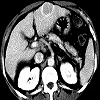
\includegraphics[height=1.0in]{../data/tomo.png}
        \caption{Tomografía 1 \footnote{Archivo tomo.png}}
    \end{subfigure}
    ~ 
    \begin{subfigure}[t]{0.3\textwidth}
        \centering
        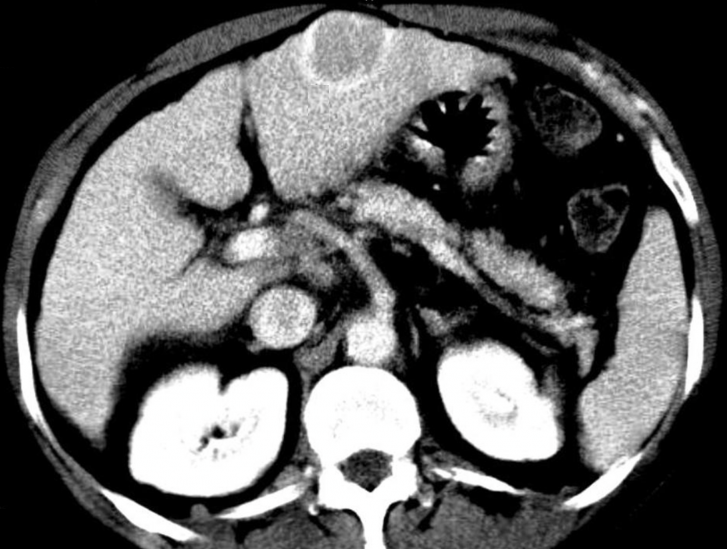
\includegraphics[height=1.0in]{../data/tomo2.png}
        \caption{Tomografía 2 \footnote{Archivo tomo2.png}}
	\label{tomo:2}
    \end{subfigure}
    ~ 
    \begin{subfigure}[t]{0.3\textwidth}
        \centering
        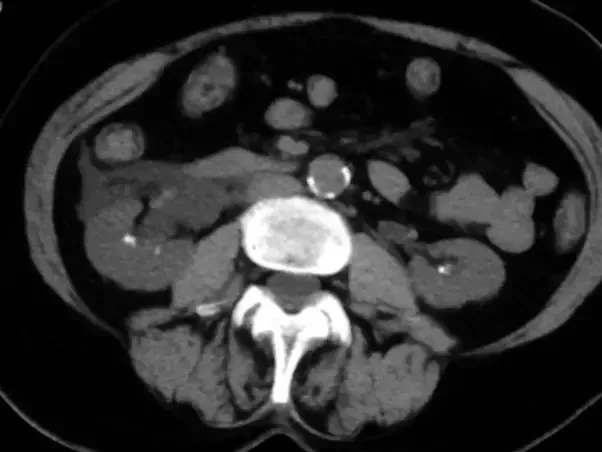
\includegraphics[height=1.0in]{../data/tomo3.png}
        \caption{Tomografía 3 \footnote{Archivo tomo3.png}}
    \end{subfigure}
    \caption{Tomografías utilizadas}
	\label{fig:tomos}
\end{figure}
% TODO: hablar de nivel de discretizacion

Proponemos 4 modelos de rayos distintos, con los cuales haremos las pruebas:

\begin{itemize}
	\item Rayos aleatorios, o \textit{random}: utilizados como base.
		Nos da una idea del comportamiento de los algoritmos.
	\item Rayos rotados, o \textit{rotated}: modelan un tomógrafo en el que el emisor de rayos
		rota alrededor del objeto, lanzando rayos que pasan por el centro del mismo. Nuestro modelo de rayos no nos va a permitir usar este método para valores de $n$ muy altos.
	\item Rayos laterales, o \textit{lateralBorders}: modela un tomógrafo en el que los rayos surgen
		desde focos a la derecha y a la izquierda de las imágenes.
	\item Rayos de todos los bordes, o \textit{allBorders}: modela un tomógrafo en el que los rayos surgen
		desde focos en los cuatro lados de la imagen.
\end{itemize}

Decidimos usar valores de \verb|n| que sean múltiplos de las imágenes originales para la experimentacion. El método de la potencia lo corrimos con 100 iteraciones como mencionamos en la sección \ref{sec:desarrollo-svd}.

% TODO: poner imagen que ilustre los rayos?
% TODO: contar que numero de iteraciones usamos en el metodo de la potencia?

\subsection{Métricas}
\label{sec:exp-metrics}

Para medir la efectividad de nuestras reconstrucciones,
se utiliza como métricas el Error Cuadrático Medio (ECM o MSE por sus siglas en inglés)
y la Proporción Máxima de Señal a Ruido (PSNR).

\begin{equation*}
   \verb|PSNR| = 10 \times \log_{10}(\verb|MAX|^2_{u}/\verb|ECM|)
\end{equation*}

donde $\verb|MAX|^2_{u}$ define el rango máximo de la imagen y \verb|ECM| es el error cuadrático medio donde se compara la imagen ideal a la imagen reconstruida.\\


Dado que utilizaremos discretizaciones de tamaño mucho menor al de las imágenes originales,
para poder compararlas con nuestras reconstrucciones,
reducimos las dimensiones de las imágenes originales utilizando \textit{GIMP}\footnote{GNU Image Manipulation Program https://www.gimp.org/}.
Estas imágenes reducidas \textbf{solamente son usadas para comparar},
nunca como \textit{input} para la simulación.

\subsection{Experimentación sobre nivel de ruido y discretización}
\label{sec:exp-noise}

Como contamos en la sección \ref{sec:desarrollo-noise},
consideramos de interés ver cómo se comporta nuestro modelo frente a distintos niveles de ruido.

Decidimos probar con ruido nulo para saber cual es la mejor métrica que se podría llegar a tener,
a pesar de que utilizando instrumentos de medición reales, este caso no existe.
Además utilizamos valores extremadamente altos de ruido para ver qué sucede en estos casos.
Nuestra hipótesis es que a medida que suba el ruido, empeoren las métricas.

En particular, a partir de cierto nivel de ruido (que esperamos cercano al 3\%),
las reconstrucciones deberían dejar de tener sentido, acercándose a un techo en el \textit{ECM}.
Para realizar estos experimentos, decidimos que la relación rayos/pixeles sea de aproximadamente 2.

% TODO: graficos? sucedio? tire fruta?
% Nombrar que algunos no pudieron conseguir todos los eigenvalues
\begin{figure}[H]
    \centering
    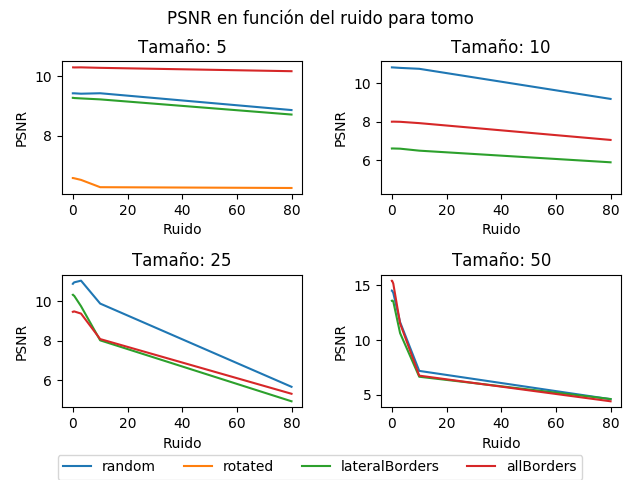
\includegraphics[width=\textwidth]{../graficos/noise/tomo/noise_graph.png}
    \caption{PSNR con respecto a la cantidad de ruido para distintos tamaños de discretización de tomo.png}
    \label{fig:exp-noise-tomo}
\end{figure}

En la figura \ref{fig:exp-noise-tomo}, podemos ver que el ruido afecta más cuanto mayor tamaño de discretización usamos.
% TODO: why?
En los tamaños 5 y 10 de \textit{tomo}, el PSNR parece prácticamente no verse modificado por este.
Sin embargo, con discretizaciones de mayor tamaño,
vemos que el ruido tiene un mayor efecto en las métricas,
principalmente a partir del 10\% de ruido.

También podemos ver que la generación aleatoria de rayos es la mejor con los tamaños del medio (10 y 25),
aunque pasando a la discretización de 50 esta ventaja desaparece.
El método de rayos rotados solo pudo usarse para $n=5$ ya que nuestro modelo de rayos
no nos permite tener la cantidad necesaria para poder probar con mayores \verb|n|
en una imagen con tan poco tamaño original (tomo.png solo mide 100x100 px).

Otra cosa destacable es que recién a partir de la discretización de 50 se puede ver una mejora
en el PSNR, llegando a valores mayores a 15 para ruidos bajos.

\begin{figure}[H]
    \centering
    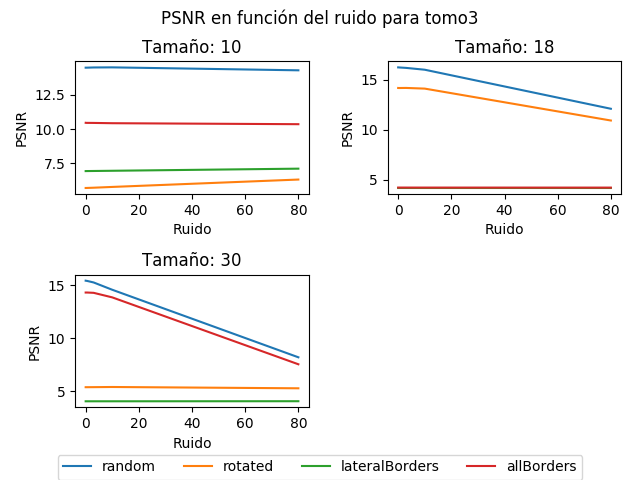
\includegraphics[width=\textwidth]{../graficos/noise/tomo3/noise_graph.png}
    \caption{PSNR con respecto a la cantidad de ruido para distintos tamaños de discretización de tomo3.png}
    \label{fig:exp-noise-tomo3}
\end{figure}

En la figura \ref{fig:exp-noise-tomo3} vemos que el método random es el mejor en todos. Cuando el tamaño es 10 no podemos decir mucho del ruido. Pero luego, para los demás tamaños, vemos que el \verb|PSNR| disminuye a medida que aumentamos el ruido. También podemos observar que a media que aumentamos el tamaño de \verb|n|, los valores de \verb|PSNR| van siendo más similares entre los distintos métodos de rayos. En líneas generales, los resultados son parecidos la figura \ref{fig:exp-noise-tomo}. 

Experimentamos con la tomografía 2 de la figura \ref{fig:tomos} y los resultados dieron también similares a las figuras \ref{fig:exp-noise-tomo} y \ref{fig:exp-noise-tomo3}. No lo incluimos para no repetirnos.


Por lo tanto, podemos concluir que el tamaño de la imagen original no varía en como afecta el ruido al \verb|PSNR|.

A continuación, vemos visualmente cómo se ve la reconstrucción:

\begin{figure}[H]
	\centering
    \begin{subfigure}[t]{0.3\textwidth}
        \centering
        
\includegraphics[height=1.0in]{img/noise/1.png}
        \caption{Tomografía size 10}
    \end{subfigure}
    ~ 
    \begin{subfigure}[t]{0.3\textwidth}
        \centering
        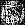
\includegraphics[height=1.0in]{img/noise/2.png}
        \caption{Tomografía size 25}
	\label{tomo:2}
    \end{subfigure}
    ~ 
    \begin{subfigure}[t]{0.3\textwidth}
        \centering
        
\includegraphics[height=1.0in]{img/noise/3.png}
        \caption{Tomografía size 50}
    \end{subfigure}
    \caption{Tomografías reconstruidas del tomo.png con el método random con ruido 0.1}
	\label{fig:resultados-noise1}
\end{figure}

\begin{figure}[H]
	\centering
    \begin{subfigure}[t]{0.3\textwidth}
        \centering
        
\includegraphics[height=1.0in]{img/noise/4.png}
        \caption{Tomografía size 10}
    \end{subfigure}
    ~ 
    \begin{subfigure}[t]{0.3\textwidth}
        \centering
        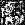
\includegraphics[height=1.0in]{img/noise/5.png}
        \caption{Tomografía size 25}
	\label{tomo:2}
    \end{subfigure}
    ~ 
    \begin{subfigure}[t]{0.3\textwidth}
        \centering
        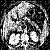
\includegraphics[height=1.0in]{img/noise/6.png}
        \caption{Tomografía size 50}
    \end{subfigure}
    \caption{Tomografías reconstruidas del tomo.png con el método allBorders con ruido 0.1}
	\label{fig:resultados-noise2}
\end{figure}

Se puede ver visualmente que el método random hizo mejor trabajo en reconstruir la imagen.
Esto puede darse ya que nuestra elección arbitraria de rayos haga que se tenga mucha información
de ciertos lugares, y menos de otros, cosa que no sucede al \textit{randomizar} los rayos.


\subsection{Experimentación sobre cantidad de rayos y discretización}
\label{sec:exp-rays}
Además, creemos importante ver cómo la relación rayos/pixeles varía la calidad de los resultados.
A nivel computacional, esto es relevante dado que a mayor cantidad de rayos, mayor tiempo de cómputo,
pero además, si se piensa en el caso de uso de un tomógrafo real,
emitir más rayos implica mayor radiación y peligro para el paciente.

Nuestra hipótesis es que la calidad de las reconstrucciones aumentará con la cantidad de rayos,
hasta un punto en el que se amesetará y dejará de crecer, por las limitaciones del método utilizado.

\begin{figure}[H]
    \centering
    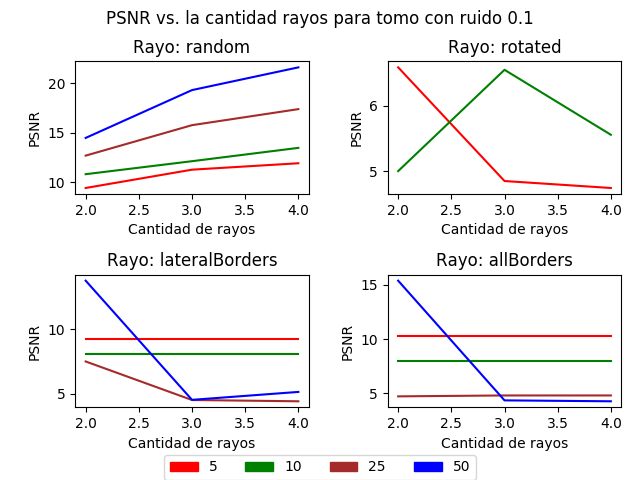
\includegraphics[width=\textwidth]{../graficos/ray_params/tomo/noise_graph_0.png}
    \caption{PSNR con respecto a la relación cantidad de rayos/cantidad de pixeles para distintos tamaños de discretización de tomo.png}
    \label{fig:exp-rayN-tomo}
\end{figure}

Como se puede ver en la figura \ref{fig:exp-rayN-tomo} para el método random estamos en lo cierto. A medida que aumentamos los rayos el \verb|PSNR aumenta|. Lo que no podemos observar es que este valor baje como esperábamos a partir de cierta cantidad de rayos. 

Luego para el resto de los métodos el \verb|PSNR| varia de maneras distintas y es bastante menor que en el random. 

La rotación de rayos podemos ver que no tiene tan buenos resultados comparándola con los otros métodos.
Además, solo lo pudimos correr para un $n=10$ y $n=5$ ya que nuestro modelo de rayos no nos permite tener la cantidad necesaria para poder probar con mayores \verb|n|.

En los últimos dos métodos restantes se observa que agregar más rayos no varia en la imagen final, salvo con $n = 50$. Esto puede pasar gracias a que siempre los rayos están cubriendo gran parte de la imagen necesaria para poder reconstruirla, ya que no son random y están ubicados de forma arbitraria. 

Si se aumenta el n, estamos dejando más celdas en la imagen libres donde puede pasar rayos.
Esto puede justificar por qué con $n = 50$ da mejor \verb|PSNR| en los métodos \verb|allBorders| y \verb|lateralBorders|.
Además puede estar pasando que a medida que se agregan más rayos en lugares fijos a la imagen,
esta se empieze a describir de mala manera y pierda \verb|PSNR|.
Se puede ver que valor de \verb|PSNR| final con $n = 50$ es parecido al del método de rotar.

También vemos el grafico del \verb|tomo3.png| que es un poco distinto al \verb|tomo.png|:

\begin{figure}[H]
    \centering
    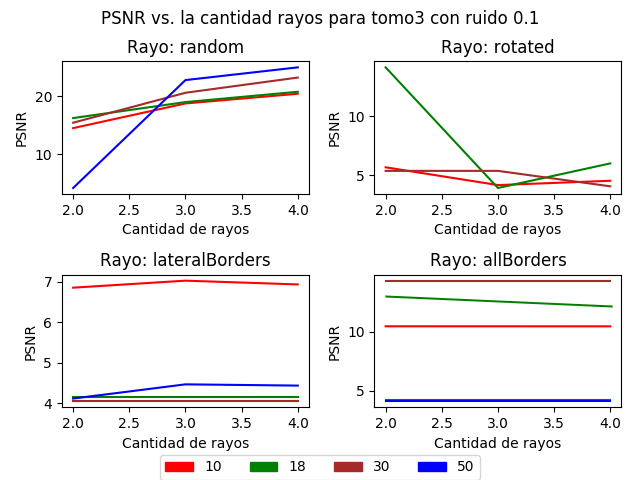
\includegraphics[width=\textwidth]{../graficos/ray_params/tomo3/noise_graph_0.png}
    \caption{PSNR con respecto a la relación cantidad de rayos/cantidad de pixeles para distintos tamaños de discretización de tomo3.png}
    \label{fig:exp-rayN-tomo3}
\end{figure}

En la figura \ref{fig:exp-rayN-tomo3} se puede observar lo mismo en el método random que en la figura     \ref{fig:exp-rayN-tomo}. A medida que aumentamos los rayos el \verb|PSNR| aumenta. Lo que no podemos observar es que este valor baje como esperábamos a partir de cierta cantidad de rayos. También podemos ver en los últimos 2 métodos que agregar más rayos no varía en la imagen final como vimos en la mayoría de los $n$ como en la experimentación anterior. Lo que se puede ver diferente es el método de rotar para $n = 18$, el \verb|PSNR| es más alto que el del método \verb|lateral borders| y parecido al del método \verb|all borders|. Esto parece indicar que la imagen es descripta de mejor manera por los rayos giratorios que tienen forma parecida a los rayos que genera  \verb|all borders|.

Veamos ahora visualmente cómo se reconstruyó una imagen variando la cantidad de rayos:

\begin{figure}[H]
	\centering
    \begin{subfigure}[t]{0.3\textwidth}
        \centering
        
\includegraphics[height=1.0in]{img/ray_n/1.png}
        \caption{Tomografía 150\% del size de rayos}
    \end{subfigure}
    ~ 
    \begin{subfigure}[t]{0.3\textwidth}
        \centering
        
\includegraphics[height=1.0in]{img/ray_n/2.png}
        \caption{Tomografía 200\% del size de rayos}
	\label{tomo:2}
    \end{subfigure}
    ~ 
    \begin{subfigure}[t]{0.3\textwidth}
        \centering
        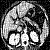
\includegraphics[height=1.0in]{img/ray_n/3.png}
        \caption{Tomografía 300\% del size de rayos}
    \end{subfigure}
    \\
    \begin{subfigure}[t]{0.3\textwidth}
        \centering
        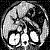
\includegraphics[height=1.0in]{img/ray_n/4.png}
        \caption{Tomografía 400 \% del size de  rayos}
    \end{subfigure}
    ~ 
    \begin{subfigure}[t]{0.3\textwidth}
        \centering
        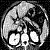
\includegraphics[height=1.0in]{img/ray_n/5.png}
        \caption{Tomografía 500 \% del size de rayos}
    \end{subfigure}
    \caption{Tomografías reconstruidas del tomo.png con el método random con ruido 0.1 de tamaño 50 variando la cantida de rayos}
	\label{fig:resultados-noise1}
\end{figure}

Se puede observar mucha diferencia reconstruyendo entre el 150\% del size de la imagen y entre el 200\% de cantidad de rayos. Luego se ve que la imagen va mejorando a medida que se aumenta la cantidad de rayos pero de manera menos drástica.

% Gráficos de calidad
% Gráficos de tiempo
% Relacion calidad/tiempo?

\subsection{Experimentación sobre cantidad de valores singulares}
\label{sec:exp-eigenvalues}
Como vimos en la sección \ref{sec:exp-noise}, algunas veces, por inestabilidad numérica
o por las propiedades de los rayos, no se pueden encontrar todos los valores singulares.
Pero, dado que estos son los más cercanos a 0, surge el interés de calcular solo los
valores singulares de mayor valor absoluto, que son los que más información nos proveen.
% Agregar en intro teorica cosas sobre low rank approximation y citarlas aca

Esperamos que las métricas bajen al bajar la cantidad de valores singulares.
Sin embargo, nuestra hipótesis consistirá en que esto solo se dará de forma
muy paulatina al principio (dado que la información descartada es poco relevante),
hasta cierto punto en el que las métricas caerán de forma más drástica,
ya que se estará perdiendo información realmente importante.

\begin{figure}[H]
    \centering
    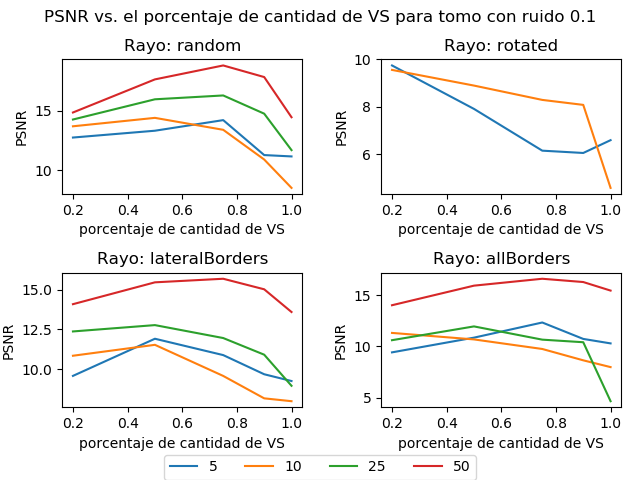
\includegraphics[width=\textwidth]{../graficos/eigens/tomo/noise_graph_2.png}
    \caption{PSNR con respecto al porcentaje de autovalores que calculamos, para distintos tamaños de discretización de tomo.png}
    \label{fig:exp-eigen-tomo}
\end{figure}

Luego de experimentar, notamos que nuestras hipótesis eran erradas.
Como podemos ver en la figura \ref{fig:exp-eigen-tomo}, en general,
dejar de lado algunos autovalores puede incluso hacer que suba el PSNR.
Tanto en el caso de los rayos random, como lateralBorders y allBorders,
suelen alcanzar máximo PSNR al utilizar solo el 75\% de los valores singulares.
Esto puede tener que ver con que los últimos autovalores calculados
arrastran los pequeños errores de muchas iteraciones de deflación,
haciendo que el resultado del Método de la Potencia de resultados que no debería teóricamente.

Sin embargo, hay excepciones.
Con los rayos rotados\footnote{Solo pudimos correr con 2 tamaños de discretización
por las mismas razones que comentamos en los experimentos anteriores},
se puede ver que alcanza máximo calculando muy pocos valores singulares.
Lo mismo sucede en algunos experimentos con otros rayos, con los tamaños de discretización más pequeños.
Intuimos que esto tiene relación con que la cantidad de información a reconstruir es mucho menor,
por lo que los primeros valores singulares son los que realmente da información, mientras que el resto solo agrega ruido.

\subsection{Experimentación sobre tiempo de valores singulares}
Viendo los efectos que tiene la cantidad de autovalores calculados,
nos interesa ver el costo computacional que tiene.
Como vimos en la sección \ref{sec:desarrollo-svd},
calcular cada autovalor tiene un costo de $O(n^2 * 100)$,
dado que hacemos 100 iteraciones con el Método de la Potencia.
Por esto, nuestra hipótesis es que el tiempo aumenta en función de la cantidad de valores singulares a calcular,
en forma cuadrática.

Para comprobarlo, corremos 20 veces nuestro programa con distintos tamaños de discretización
sobre la imagen tomo.png, y tomamos el promedio del tiempo entre el principio y el final del cálculo de CML.
\begin{figure}[H]
    \centering
    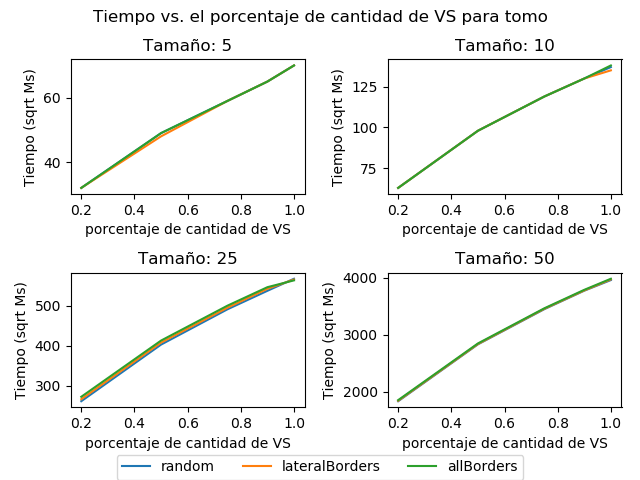
\includegraphics[width=\textwidth]{../graficos/eigens-time/tomo/noise_graph.png}
    \caption{Tiempo de cálculo de CML en función del porcentaje de valores singulares a calcular para tomo.png 
    (escala con raíz cuadrada en el eje vertical)}
    \label{fig:exp-eigenvalues-time}
\end{figure}

Como se puede ver en la figura \ref{fig:exp-eigenvalues-time},
a medida que aumentan la cantidad de valores singulares que deseamos calcular,
también aumenta el tiempo de cómputo para conseguirlo.
Notar que la escala tiene raíz cuadrada en el eje vertical.
Viendo que queda una función prácticamente lineal,
comprobamos que el crecimiento es cuadrático.
Esto comprueba lo que vimos teóricamente.

Con estos resultados, concluimos que es mejor acotar la cantidad de valores singulares a tomar,
ya que permite mejorar las reconstrucciones ahorrando una gran cantidad de tiempo.


\subsection{Experimentación sobre el tamaño de la imagen de salida}
Dados muchos de los resultados anteriores, se nos hace muy interesante enfatizar lo que sucede con la calidad de los resultados
en variación del tamaño de la imagen de salida. Nos interesa saber si efectivamente tamaños más grandes dan como resultado
\verb|PSNR| mayor, y si en algun punto este crecimiento se estanca y resulta innecesario el cálculo de tamaños muy grandes.
Nuestra hipótesis es que a medida que el tamaño aumente, así seguirá el \verb|PSNR|.

\begin{figure}[H]
    \centering
    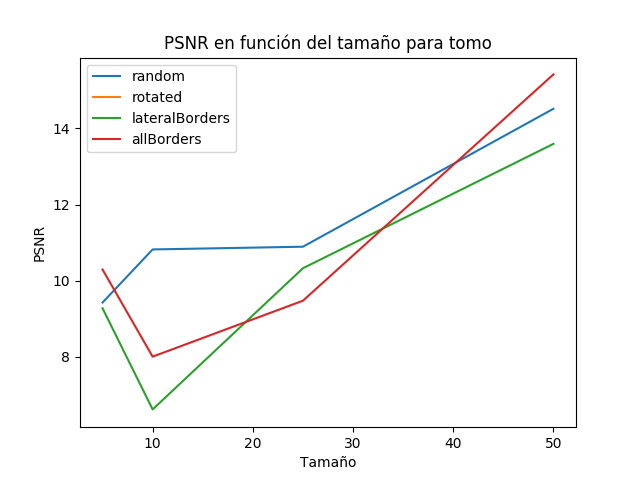
\includegraphics[width=\textwidth]{../graficos/size/tomo/noise_graph.png}
    \caption{PSNR en función del tamaño de la imagen de salida para tomo.png}
    \label{fig:exp-size-1}
\end{figure}

Se puede ver en la figura \ref{fig:exp-size-1} como al aumentar el tamaño de la imagen, también hace crecer el \verb|PSNR|.
% La explicación más directa para este resultado, también es la intuitiva: a más resolución, mejor calidad.
% Sin embargo,  con una explicación más profunda podemos decir que al tener mayor tamaño,
% también tenemos más pixeles de donde sacar información, y estos nos resultan como ecuaciones para nuestras incognitas.
% Por lo que tiene sentido que mayor tamaño den mejores resultados.
Creemos que esto se debe a que al usar discretizaciones muy pequeñas,
se hace que un pixel de la reconstrucción utilice información
de pixeles muy variados de la imagen original,
haciendo que no se parezca en nada a esta.

Algo interesante para destacar, es que si miramos en la figura \ref{fig:exp-eigenvalues-time} podemos ver que mayores tamaños también resultan en
mayor tiempo de cómputo\footnote{En nuestra experiencia con imágenes grandes (90x90), tardan mucho, incluso más de 12hs}. 
Nos encontramos entonces con un \textit{trade-off} entre tiempo y calidad.

\section{Conclusiones}
\label{sec:conclusiones}

Se nos pidió implementar un programa en lenguaje C++ que simule el proceso de una tomografía computada y su reconstrucción, que realice el procedimiento explicado en el enunciado del trabajo práctico.


Para la correcta resolución del mismo utilizamos uno de los métodos de aproximación visto en clase, cuadrados mínimos lineales y fuimos capaces de aplicar los conceptos teóricos que este método propone al problema práctico de reconstruir una imagen, que pudiera estar sujeta a ruido.


Durante el desarrollo y la resolución del mismo observamos el gran potencial del método para este tipo de problemas. No obstante, vimos que el método trae de la mano un gran problema de estabilidad numérica, como se discutió en la sección anterior, lo cual puede traer altercados a la hora de realizar los cálculos necesarios.


Con el fin de solventar los problemas de estabilidad numérica, se propuso la utilización de la descomposición SVD de la matriz asociada al sistema lineal a resolver. 


De esta manera, fuimos capaces de observar el impacto que tuvo la aplicación de la descomposición vista en clase a la hora de aminorar estos conflictos, pues como se vio en la materia y se discutió en la sección anterior el número de condición de las matrices ortogonales ($U$ y $V$) es el mínimo posible y en el caso de la matriz diagonal ($\Sigma$) no se requiere realizar Eliminación Gaussiana.


Teniendo esto en mente, pudimos hacer uso de un buen método de aproximación, cuadrados mínimos lineales, sin tener que pagar el costo de su inestabilidad numérica.\\

En la experimentación no vimos diferencias notorias que valgan la pena mencionar cuando probamos con distintas imágenes. Esto nos hace concluir que es un método genérico que funciona para distintos casos.

Además probamos con distintas formas de generar rayos para reconstruir la imagen. Pudimos ver que el método más
eficiente fue el de generar los rayos de manera aleatoria, en la mayoría de los casos. Seguido por los métodos de
all borders y lateral borders. Y por último el método de rotar, que no dió buenos resultados en casi ningún experimento.
Llegamos a la conclusión que el método de rotar no funciona de manera eficiente porque queda mucha área en la imagen sin 
cubrir por rayos. También pensamos que el método \verb|all borders| y \verb|lateral borders| funciona peor en la mayoría de 
los casos porque tienen una estructura definida y limitada que se repite de igual manera para todas las imágenes. 
Esto puede hacer que deje afuera ciertos datos importantes para algunas imágenes.

También experimentamos con distinta cantidad de rayos en función de los distintos tamaños de nuestras imágenes de prueba, y conseguimos
resultados muy interesantes. Concluimos que no necesariamente aumentar la cantidad de rayos aumenta la calidad del resultado, como sería 
intuitivo pensar, sino que es una variable que está muy determinada por el método de generación de rayos que se está empleando.

Luego hicimos experimentos variando la cantidad de valores singulares que calculamos para resolver CML y llegamos a conclusiones bastante 
inesperadas en comparación a otros experimentos. Nuestra hipótesis inicial era que cuanto mayor sea el número de valores singulares se 
calculen, mejor sería la calidad de los resultados. Sin embargo nos encontramos con que hay un limite para este número, donde la calidad de los 
resultados empieza a decrecer. Con esto concluimos que la cantidad de valores singulares es muy útil hasta cierto punto donde se tiene más 
información que la necesaria para resolver el problema, y comienza a perjudicar en la calidad de los resultados.

Por último, también nos fue de interés experimentar con los tiempos de cómputo. Como es muy usual en este tipo de problemas, nuevamente 
nos encontramos con un \textit{trade-off} entre la velocidad con la que se pueden obtener resultados, y la calidad ó confiabilidad 
de los mismos, a la hora de elegir el tamaño de la discretización. En este trabajo se pudo experimentar de primera mano la enorme cantidad de tiempo que puede llevar resolver un problema 
computacional, y podemos concluir que este \textit{trade-off} se debe tener muy presente a la hora de aplicar estos resultados en la 
práctica.

% Documentacion: https://en.wikibooks.org/wiki/LaTeX/Bibliography_Management
\section{Referencias}
\begin{thebibliography}{9}
\bibitem{burdenSVD}
R. L. Burden y J.D.Faires, \textit{Numerical Analysis (2011)}, Ninth Edition. p. 614 (9.6 Singular Value Decomposition)

\bibitem{pot}
R. L. Burden y J.D.Faires, \textit{Numerical Analysis (2011)}, Ninth Edition. p. 576 (9.3 The Power Method)

\bibitem{lowrank}
N. Truhar y B. Dukic, \textit{Low rank approximation using singular value decomposition}

\end{thebibliography}
\appendix

\section{Enunciado}
\label{ap:enunciado}
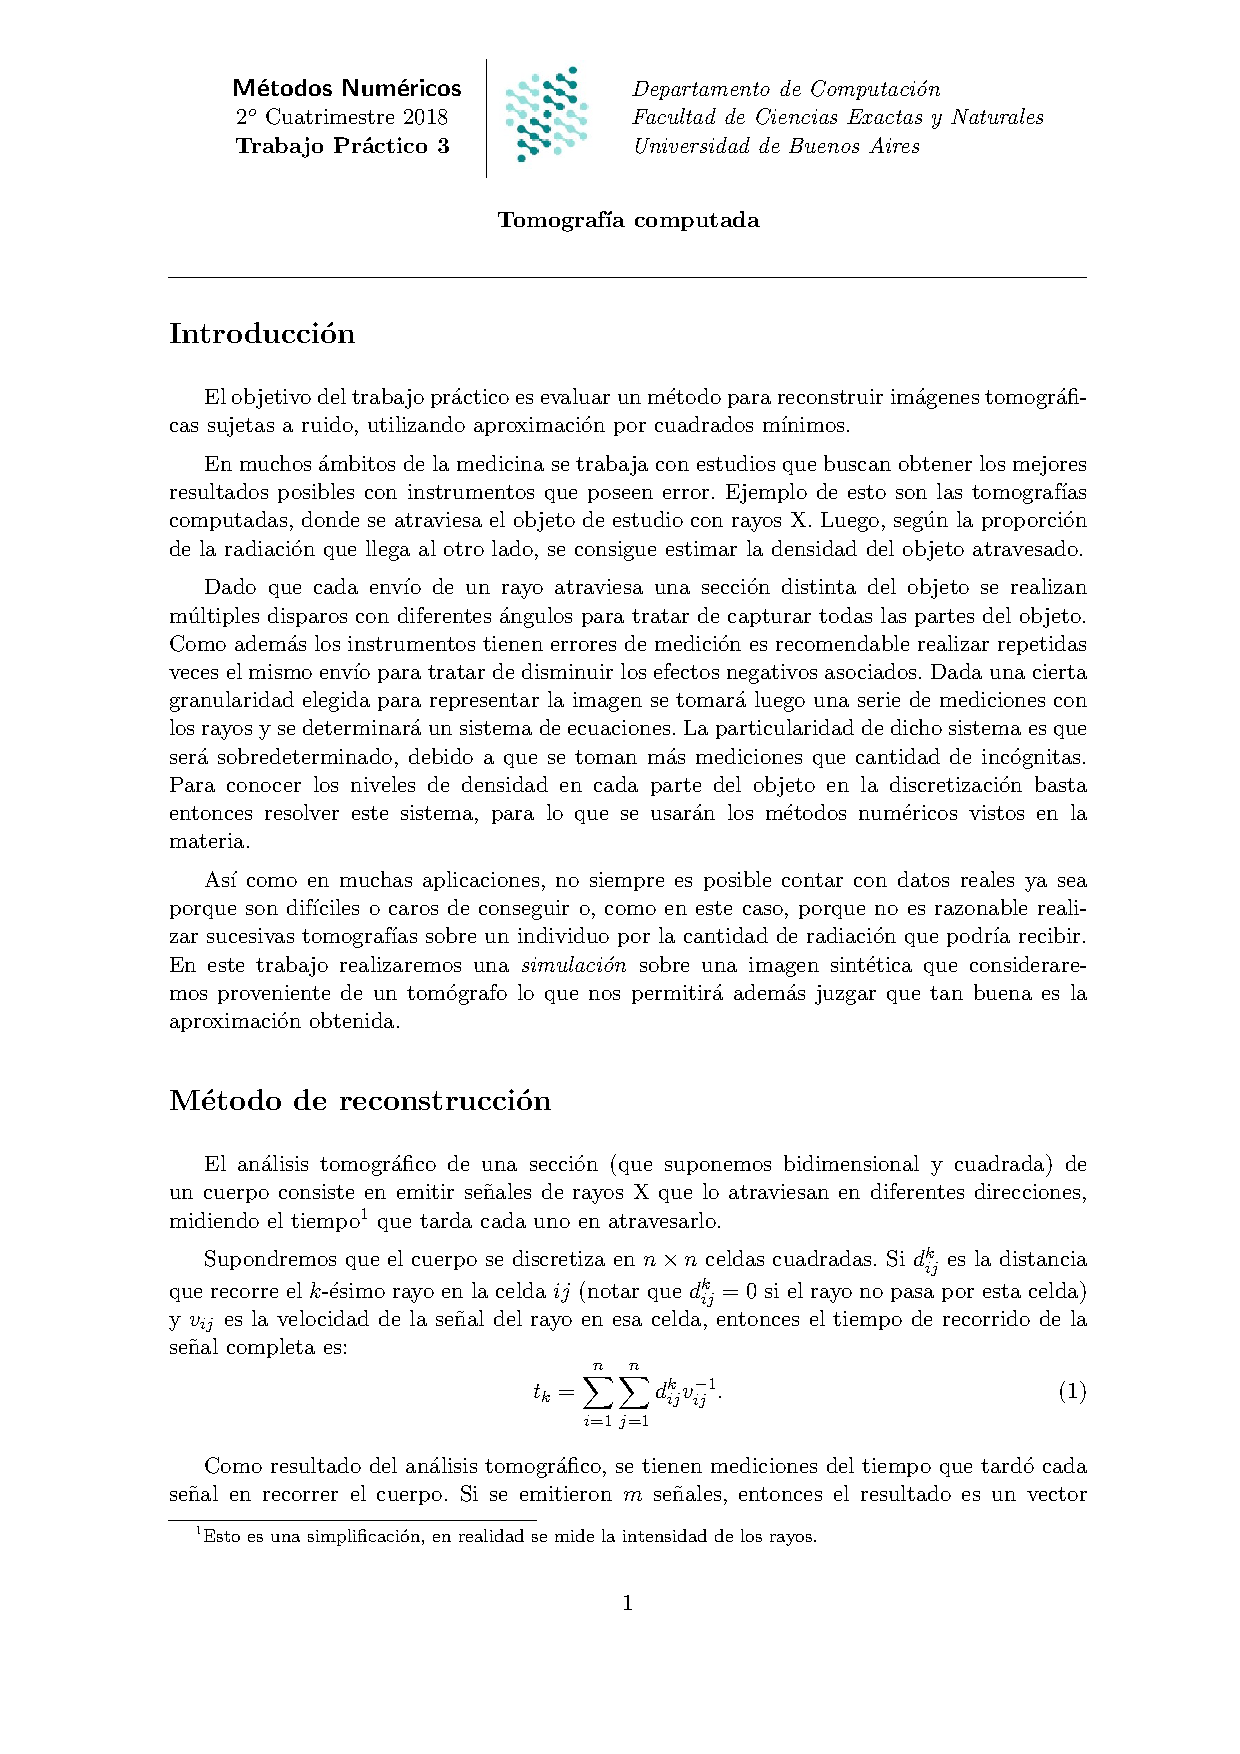
\includepdf[pages=-]{../enunciado/tp3.pdf}

\section{Código fuente relevante numéricamente}

Código del Método de la Potencia:
\begin{lstlisting}
double metodoPotencia(
    const std::vector<std::vector<double>> &A,
    std::vector<double> &v,
    int numeroIteraciones) {
    obtenerVectorRandom(v);

    for (int iteracion = 0; iteracion < numeroIteraciones; iteracion++) {
        v = normalizar(A * v);
    }
    return (v * (A * v)) / (v * v);
}
\end{lstlisting}
\end{document}
